% !TeX root = RJwrapper.tex
\title{R package learningtower: Exploring standardised test scores
across the globe}
\author{by Priya Ravindra Dingorkar, Kevin Wang, and Di Cook}

\maketitle

\abstract{%
An abstract of less than 150 words - Discuss what the paper talks about
with a little introduction.
}

\hypertarget{introduction}{%
\section{Introduction}\label{introduction}}

The Organization for Economic Cooperation and Development
\href{OECD\%20-\%20https://www.oecd.org/about/}{OECD} is a global
organization that aims to create better policies for better lives. Their
mission is to create policies that promote prosperity, equality,
opportunity, and well-being for all.

\href{PISA\%20-\%20https://www.oecd.org/pisa/}{PISA} is one of the
OECD's Programme for International Student Assessment. PISA assesses
15-year-olds potential to apply their knowledge and abilities in
reading, mathematics, and science to real-world challenges. The OECD
launched this in 1997, it was initially administered in 2000, and it
currently includes over
\href{https://www.oecd.org/pisa/aboutpisa/pisa-participants.htm}{80
nations}. The PISA study, conducted every three years, provides
comparative statistics on 15-year-olds performance in reading, maths,
and science.

\hypertarget{what-is-pisa}{%
\section{What is PISA?}\label{what-is-pisa}}

PISA assesses the extent to which children approaching the end of
compulsory school have learned some of the information and abilities
required for full participation in modern society, notably in maths,
reading, and science. The examination focuses on reading, mathematics,
science, and problem solving. It also assesses students capacity to
replicate information and extrapolate from what they have learned and
apply that knowledge in unexpected circumstances, both inside and
outside of school. This approach reflects the fact that individuals are
rewarded in modern economies not for what they know, but for what they
can accomplish with what they know.

This evaluation, which is carried out every three years, assists in
identifying students development of knowledge and skills throughout the
world, which can provide actionable insights and therefore assist
education policymakers. PISA is well known for its distinctive testing
characteristics, which include policy orientation, an innovative notion
of literacy, relevance to lifelong learning, regularity, and breadth of
coverage. PISA is now used as an assessment tool in many regions around
the world. In addition to OECD member countries, the survey has been or
is being conducted in East, South and Southeast Asia, Central,
Mediterranean and Eastern Europe, and Central Asia, The Middle East,
Central and South America and Africa.

For each PISA, one domain is thoroughly examined. In 2018, for example,
reading was assessed alongside mathematics and science as minor areas of
assessment. The 2012 survey concentrates on mathematics, with reading,
science, and problem solving serving as minor evaluation topics.

PISA targets a certain age group of pupils in order to properly compare
student performance worldwide. PISA students are aged between 15 years 3
months and 16 years 2 months at the time of the assessment, and have
completed at least 6 years of formal schooling. They can enroll in any
sort of institution, participate in full-time or part-time education,
academic or vocational programs, and attend public, private, or
international schools inside the country. Using this age across nations
and throughout time allows PISA to compare the knowledge and abilities
of people born in the same year who are still in school at the age of
15, irrespective of their diverse schooling.

\hypertarget{r-package---learningtower}{%
\section{R package - learningtower}\label{r-package---learningtower}}

\hypertarget{data-description}{%
\section{Data Description}\label{data-description}}

\hypertarget{data-compilation}{%
\subsection{Data Compilation}\label{data-compilation}}

\hypertarget{data-structure}{%
\section{Data Structure}\label{data-structure}}

\hypertarget{exploratory-data-analysis}{%
\section{Exploratory Data Analysis}\label{exploratory-data-analysis}}

\hypertarget{gender-analysis}{%
\section{Gender Analysis}\label{gender-analysis}}

\hypertarget{socioeconomic-factors-analysis}{%
\section{Socioeconomic Factors
Analysis}\label{socioeconomic-factors-analysis}}

\hypertarget{temoral-trend-australia}{%
\section{Temoral Trend Australia}\label{temoral-trend-australia}}

\hypertarget{future-developments}{%
\section{Future Developments}\label{future-developments}}

\hypertarget{summary}{%
\section{Summary}\label{summary}}

\hypertarget{testing}{%
\section{Testing}\label{testing}}

Figure @ref(fig:penguins-ggplot) shows an plot of the
\CRANpkg{palmerpenguins} data \citep{palmerpenguins}, made using the
\CRANpkg{ggplot2} package. This data features three penguin species
which has a lovely illustration by Alison Horst in Figure
@ref(fig:penguins-alison).

\begin{Schunk}
\begin{Sinput}
penguins %>%
  ggplot(aes(x = bill_depth_mm, y = bill_length_mm,
             color = species)) +
  geom_point()
\end{Sinput}
\begin{figure}
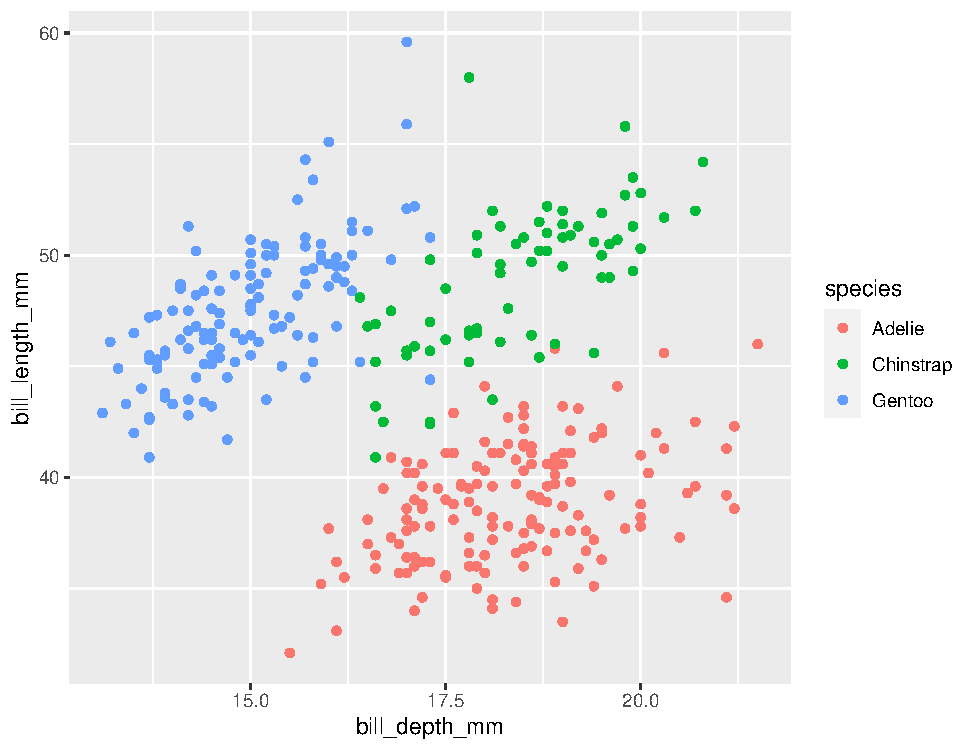
\includegraphics{learningtower_files/figure-latex/penguins-ggplot-1} \caption[A basic non-interactive plot made with the ggplot2 package on palmer penguin data]{A basic non-interactive plot made with the ggplot2 package on palmer penguin data. Three species of penguins are plotted with bill depth on the x-axis and bill length on the y-axis. Visit the online article to access the interactive version made with the plotly package.}\label{fig:penguins-ggplot}
\end{figure}
\end{Schunk}

\citet{RJ-2021-050}

We have displayed various tooltips that are available in the package
\pkg{ToOoOlTiPs}.

\bibliography{learningtower.bib}

\address{%
Priya Ravindra Dingorkar\\
Monash University\\%
Department Econometrics and Business Statistics\\ Clayton, Australia\\
%
\url{https://www.linkedin.com/in/priya-dingorkar/}\\%
%
\href{mailto:priyadingorkar@gmail.com}{\nolinkurl{priyadingorkar@gmail.com}}%
}

\address{%
Kevin Wang\\
University of Sydney\\%
School of Mathematics and Statistics\\ Sydney, Australia\\
%
\url{https://kevinwang09.github.io/}\\%
%
\href{mailto:kevinwangstats@gmail.com}{\nolinkurl{kevinwangstats@gmail.com}}%
}

\address{%
Di Cook\\
Monash University\\%
Department Econometrics and Business Statistics\\ Clayton, Australia\\
%
\url{http://dicook.org/}\\%
%
\href{mailto:dicook@monash.edu}{\nolinkurl{dicook@monash.edu}}%
}
